\chapter{Riferimenti Storici}\label{chap:riferimentiStrotici}

%\section{Introduzione} \label{sec:riferimentiStorici}
%Cosa posso inserire?

\section{BlockSci} \label{sec:riferimentiStorici}

BlockSci è un software open source di analisi delle blockchain basate sull'organizzazione dati di Bitcoin scritto in C++; sviluppato dall'Università di Princeton, offre un metodo di analisi della blockchain di Bitcoin attraverso l'estrazione di dati utilizzando il framework RPC di Bitcoin-core e l'utilizzo di un parser per l'analisi delle informazioni serializzate dal nodo Bitcoin.
I dati estratti vengono salvati attraverso un'organizzazione che si basa su flat-file e su database relazionale come SQLite.
In questo documento esamineremo solo il modulo relativo al parser e all'organizzazione delle informazioni estratte; BlockSci inoltre offre un evoluto sistema per l'analisi dei dati estratti con cui si ha la possibilità di costruire analisi sulla rete Bitcoin.\\
Il parser di BlockSci utilizza un metodo di lettura delle informazioni sequenziale in cui effettua una serie di ottimizzazioni per il corretto funzionamento del modulo di analisi.
Costruisce un grafo delle transazioni miniale in cui serializza le transazioni con una struttura dati illustrata nella Tabella \ref{tab:blockSciSerialization}.

\begin{table}
       \centering\small
           \begin{tabular}{|c|c|}
               \hline
                 \multicolumn{2}{|c|}{\textbf{Transaction}} \\
                 %\cmidrule(lr){1-2}
                 \hline
                 \multicolumn{1}{|c|}{Size} & \multicolumn{1}{c|}{Description} \\
               \hline \hline
               32 bit & Size   \\
               \hline
               32 bit & LockTime \\
               \hline
               16 bit & Input count \\
               \hline
               16 bit & Output count \\
               \hline
               128 bits each & Outputs \\
               \hline
               128 bits each & Inputs \\
               \hline
       \end{tabular}
       \caption{Struttura delle transazioni in BlockSci per la costruzione del grafo delle transazioni \cite{blocksci:article}.\label{tab:blockSciSerialization}}
   \end{table}

Nel ducumento \cite{blocksci:article} vengono descritte le prestazioni del parser, il quale per effettuare l'estrazione dei dati dalla blockchain di Bitcoin con una dimensione pari a 140 GB impiega 11 ore, utilizzando una cache di 8 Gb, aumentando la dimensione di quest'ultima si riescono ad ottenere prestazioni migliori.

\section{BiVA} \label{sec:biva}

BiVA (Bitcoin Network Visualization \& Analysis) è un software sviluppato dall'Università di Singapore che utilizza NEO4J per la costruzione di un grafo di address attraverso l'estrapolazione dei dati tramite il framework RPC di Bitcoin-core; inoltre implementa un algoritmo di analisi su grafo per la ricerca degli address più utilizzati all'interno della blockchain di Bitcoin.\\
Il documento \cite{biva:article} descrive prevalentemente l'algoritmo di analisi utilizzato, ma questo argomento non verrà trattato in questo documento.\\
Inoltre non vengono riportati dati sulle tempistiche di deserializzazione, neppure sul metodo in cui si effettuano le richieste delle informazioni tramite Bitcoin-core; essendo il framwork RPC, un framework non progettato per l'estrazione completa dei dati dalla blockchain, le tempistiche dovrebbero essere abbastanza elevate utilizzando un software \emph{single theread}.\\
Una porzione di grafo prodotto attraverso BiVA è rappresentato in Figura \ref{fig:bivaGraph}.

\begin{figure}
\centering
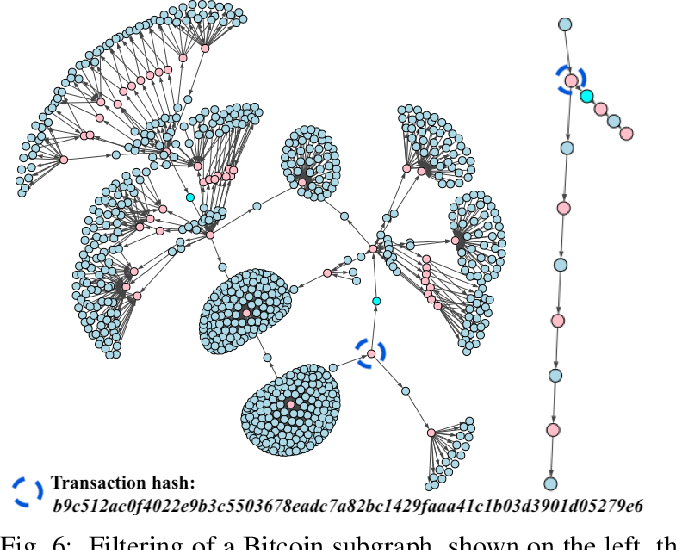
\includegraphics[scale=0.35]{images/bivaGraph.png}
\caption{Frammento del grafo degli address creato attraverso BiVA \cite{biva:article}.\label{fig:bivaGraph}}
\end{figure}


\section{Bitcoin Transaction Visualization} \label{sec:bitcoinTransactionVis}

Uno studio condotto dall'Universita di Saskatchewan e pubblicato nel articolo \cite{BitcoinBlockchainTransactionsVisualization:article} descrive la creazione di un grafo di transazioni localizzato attraverso l'utilizzo dell API di \url{https://blockchain.com}.\\
L'utilizzo di questa API ha permesso di localizzare le transazioni attraverso la sua posizione geografica grazie all'IP messo a disposione della servizio per ogni transazione (quando questo ip è esposto).\\
La demo per la dimostrazione di questo studio viene sviluppata attraverso tecnologie web con un uso estensivo di JQuery, La Figura \ref{fig:bitcoinTransactionVis} ne rappresenta un esempio.

\begin{figure}[H]
\centering
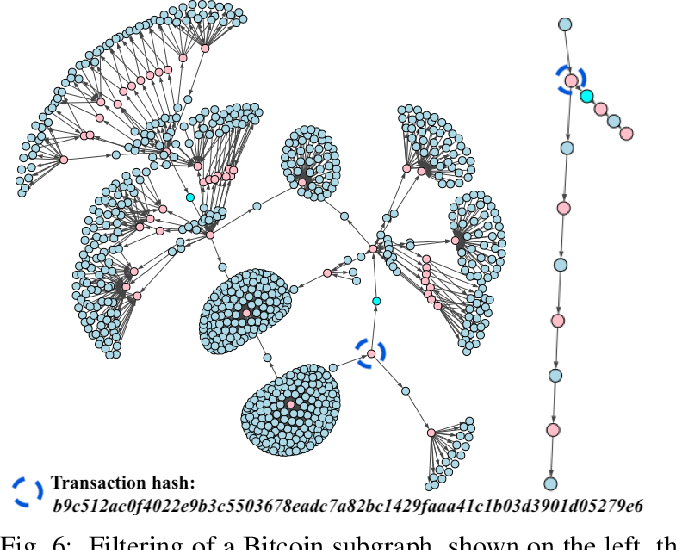
\includegraphics[scale=0.35]{images/bivaGraph.png}
\caption{Frammento del grafo di transazioni prodotto attraverso la demo pubblicata nell'articolo \cite{BitcoinBlockchainTransactionsVisualization:article}.\label{fig:bitcoinTransactionVis}}
\end{figure}
